\documentclass[aps,pra,notitlepage,amsmath,amssymb,letterpaper,12pt]{revtex4-1}
\usepackage{amsthm}
\usepackage{graphicx}
%  Above uses the Americal Physical Society template for Physical Review A
%  as a reasonable and fully-featured default template
 
%  Below define helpful commands to set up problem environments easily
\newenvironment{problem}[2][Problem]{\begin{trivlist}
\item[\hskip \labelsep {\bfseries #1}\hskip \labelsep {\bfseries #2.}]}{\end{trivlist}}
\newenvironment{solution}{\begin{proof}[Solution]}{\end{proof}}
 
% --------------------------------------------------------------
%                   Document Begins Here
% --------------------------------------------------------------
 
\begin{document}
 
\title{Classroom CW 01}
\author{Alice, Max, Keith}
\affiliation{CS510, Schmid College of Science and Technology, Chapman University}
\date{\today}

\maketitle

\section{Problem} % Specify main sections this way

% 1
\begin{problem}{1} 
Definition of the derivative $f'(x)$ of a function $f(x)$
\end{problem}

\begin{solution} %You can also use proof in place of solution
The derivative of $f(x)$ with respects to $x$ is the function $f'(x)$ and is defined as,
\begin{align}
f'(x) = \lim\limits_{x \to 0}\frac{f(x+h)-f(x)}{h}
\end{align}
% Use align environments for equations. The \\ is a newline character. The & is the alignment character.
% Using align* or \nonumber on each line removes equation numbers
\end{solution}

\subsection{Visual} % Specify subsections and subsubsections this way

Figure of Problem 1.

\begin{figure}[h!] % h forces the figure to be placed here, in the text
  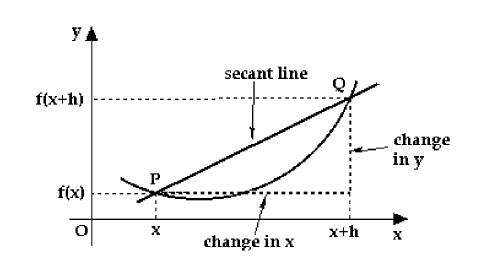
\includegraphics[width=0.7\textwidth]{limits_and_derivates.JPG}  % if pdflatex is used, jpg, pdf, and png are permitted
  \caption{Visual graph of the definition of the derivative.}
  \label{fig:figlabel}
\end{figure}

\section{References}
\noindent Dawkins, Paul (2003), \textit{Paul's Online Math Notes}
\url {http://tutorial.math.lamar.edu/Classes/CalcI/DefnOfDerivative.aspx}

\noindent Fouss, Kristen, \textit{Honors Precalc Resources}, \url{http://image.tutorvista.com/content/feed/u1989/limits and derivates.JPG}

 
\end{document}
